\documentclass{article}

% We suggest
% if you need to pass options to natbib, use, e.g.:
%     \PassOptionsToPackage{numbers, compress}{natbib}
% before loading neurips_2020

% ready for submission
%\usepackage{neurips_2020_tda}

% to compile a preprint version, e.g., for submission to arXiv, add add the
% [preprint] option:
%     \usepackage[preprint]{neurips_2020_tda}

% to compile a camera-ready version, add the [final] option, e.g.:
%     \usepackage[final]{neurips_2020_tda}

% to avoid loading the natbib package, add option nonatbib:
\usepackage[nonatbib]{neurips_2020_tda}

\usepackage[utf8]{inputenc} % allow utf-8 input
\usepackage[T1]{fontenc}    % use 8-bit T1 fonts
\usepackage{amsfonts}       % blackboard math symbols
\usepackage{booktabs}       % professional-quality tables
\usepackage{hyperref}       % hyperlinks
\usepackage{url}            % simple URL typesetting
\usepackage{microtype}      % microtypography
\usepackage{nicefrac}       % compact symbols for 1/2, etc.
\usepackage{paralist}       % in-paragraph enumerations
\usepackage{siunitx}        % SI units
\usepackage{amsmath,amssymb}
\urlstyle{same}

%HANS's CONVENIENCES
\usepackage{mymacros}
\usepackage{graphicx}

\title{Multidimensional Persistence Module Classification via Lattice-Theoretic Convolutions}

% The \author macro works with any number of authors. There are two commands
% used to separate the names and addresses of multiple authors: \And and \AND.
%
% Using \And between authors leaves it to LaTeX to determine where to break the
% lines. Using \AND forces a line break at that point. So, if LaTeX puts 3 of 4
% authors names on the first line, and the last on the second line, try using
% \AND instead of \And before the third author name.

\author{%
  Hans Riess  \\
  Department of Electrical and Systems Engineering \\
  University of Pennsylvania\\
  Philadelphia, PA 19104 \\
  \texttt{hmr@seas.upenn.edu} \\
  % examples of more authors
  \And
  Jakob Hansen \\
  Department of Mathematics \\
  Ohio State University \\
  Columbus, OH 43210 \\
  \texttt{hansen.612@osu.edu}
  % Address \\
  % \texttt{email} \\
  % \AND
  % Coauthor \\
  % Affiliation \\
  % Address \\
  % \texttt{email} \\
  % \And
  % Coauthor \\
  % Affiliation \\
  % Address \\
  % \texttt{email} \\
  % \And
  % Coauthor \\
  % Affiliation \\
  % Address \\
  % \texttt{email} \\
}

\begin{document}

\maketitle

\begin{abstract}
 Multiparameter persistent homology has been largely neglected as an input to
 machine learning algorithms.
 We consider the use of lattice-based convolutional neural network layers as a 
 tool for the analysis of features arising from multiparameter persistence
 modules. We find that these show promise as an alternative to convolutions for
 the classification of multidimensional persistence modules.
\end{abstract}

\section{Introduction}

Persistent homology has the ability to discern both the global
topology~\cite{ghrist_barcodes:_2008} and local
geometry~\cite{bubenik_persistent_2020} of finite metric spaces (e.g. embedded
weighted graphs, point clouds in $\R^d$) making it a befitting feature for the
purposes of training a neural network. Single-dimensional homological
persistence has drawn recent attention in deep learning~\cite{hofer_deep_2017,
pun_persistent-homology-based_2018, bruel-gabrielsson_topology_2020}. This is,
in part, due to a wide range of efficient software
libraries~\cite{otter_roadmap_2017, henselman_matroid_2017, bauer_ripser:_2019}
for computing persistent homology, %barcodes (in the ``west-coast'' lingo) of
% filtrations,
as well as a growing cookbook of recipes 
for featurizing barcodes from single dimensional persistence, including
persistence images~\cite{adams_persistence_2017}, persistence
landscapes~\cite{bubenik_statistical_2015}, and more exotic methods
\cite{kalisnik_tropical_2019}.

Multidimensional persistence generalizes single-dimensional persistent homology
in order to tackle filtrations parameterized in multiple dimensions.
% Such
% filtrations arise, for example, in a Rips filtration of a finite metric space
% for which the finite metric space itself carries a filter function. %is parameterized by a signal
% %attributing a vector in $\R^d$ to every point of the metric space.
% Restricting
% to points in the metric space appearing below a certain coordinate-wise
% threshold results in a multi-filtration of the corresponding Rips complexes.
%Multidimensional persistence boasts stability properties similar to those in one
%dimension~\cite{lesnick_theory_2015}.
Unfortunately, there is no complete
compact barcode-like characterization of multidimensional persistence
modules~\cite{carlsson_theory_2009}. We must make do with incomplete invariants.
There are various algebraic invariants; in this paper we will use the
\textit{Hilbert function} and the \textit{multi-graded Betti numbers}, both of
which are $\mathbb{N}$-valued functions on the parameter space.
%Their names arise from their relationship with the homological algebra of
%persistence modules.
The Hilbert function is nothing more than the pointwise
(topological) Betti numbers\footnote{\textit{Caveat lector:} the multi-graded
Betti numbers are not the same as the topological Betti numbers
$\beta_i(\mathbb{X}) = \dim(H_i(\mathbb{X}))$.}, and the multi-graded Betti
numbers have a geometric interpretation in terms of births and deaths~\cite{knudson_refinement_2008}.

% The \textit{rank
% invariant}, another invariant, is shown to be complete in the case of single
% dimensional persistence \cite{carlsson_theory_2009}; due to its difficulty to
% compute it is not considered here.

Multidimensional persistence suffers two hindrances to its usefulness in
machine learning. First, software for computing multidimensional persistence is
scarce. To the authors' knowledge, RIVET is the only available software for
computing multidimensional persistence~\cite{lesnick_interactive_2015}; RIVET
specializes to $2$-dimensional persistence and is focused on interactive
visualization rather than machine-interpretable output.
% provides a user-interface for
% visualizing multi-filtrations as well as a pipline for computing the Hilbert
% function and the multi-graded Betti numbers in degrees $0$, $1$, and $2$.
Second, %for all the attention multidimensional persistence has received,
there has been no activity, as far as the authors are aware, studying the extraction
of suitable features for multidimensional persistent homology.
%Carlsson has a little bit in a recent paper...

We hope to ignite an interest in filling both of these gaps. In this paper, we
propose a naive featurization of multidimensional persistence modules based on
the aforementioned invariants, and design an architecture for classifying these
persistence modules. This architecture employs a lattice-theoretic notion of
convolution, thereby respecting the order relation of the parameters of the
persistence module. We implement our model and compare the performance of our
proposed lattice-convolutional architecture with a (simplified) standard
convolutional architecture.

\section{Backgound}

Space constraints require that this section be laconic. For a primer on
persistent homology, see~\cite{ghrist_barcodes:_2008, carlsson_topology_2009};
for multiparameter persistent homology, see~\cite{lesnick_interactive_2015}. An
introduction to lattices may be found in~\cite{davey2002introduction}.

\subsection{Rips complexes and persistent homology}
Let $(\mathcal M,d)$ be a finite metric space. The \introduce{Vietoris-Rips
  complex} of $\mathcal M$ at scale $r$ is the abstract simplicial complex
$\text{Rips}_r(\mathcal M)$ whose simplices are subsets of $\mathcal M$ of
diameter at most $r$. There is a natural inclusion $\text{Rips}_r(\mathcal M)
\to \text{Rips}_{r'}(\mathcal M)$ for $r \leq r'$.

Applying the simplicial homology functor (with coefficients in a field $k$)
$H_i$ to $\text{Rips}_r(\mathcal M)$ produces a sequence of vector spaces
$PH_i(r)$. The inclusions $\text{Rips}_r(\mathcal M) \to
\text{Rips}_{r'}(\mathcal M)$ induce maps $PH_i(r) \to PH_i(r')$, producing the
data of \introduce{persistence module}. This structure can be compactly
described as a functor from $\R$, viewed as a category via its standard order
structure, to the category $\Vect_k$ of vector spaces over $k$. The simplicity
of the category $\R$ gives these persistence modules simple structure: they
decompose as direct sums of interval modules $I_{[a,b)}$, which have
$I_{[a,b)}(r) = k$ for $a \leq r < b$ and zero otherwise. The maps are the
identity where possible and the zero map otherwise.
% is this the right shape for the intervals?

% This representation theoretic fact gives a representation\footnote{Pun intended.} of
% $\R$-indexed persistence modules via \introduce{barcodes} or
% \introduce{persistence diagrams}. Each bar $I_{[a,b)}$ in the barcode represents
% a homology class which is \introduce{born} at $a$ and \introduce{dies} at $b$.

\subsection{Multiparameter persistence}
The Rips construction produces a filtration of simplicial complexes from a
finite metric space; it is natural to consider the behavior of the homology
functor over a pair of coherent filtrations. Consider
a finite metric space $(\mathcal M, d)$ and a filtration
function $\rho:\mathcal M \to \R$. This data specifies a bifiltration of
simplicial complexes given by
\[\mathbb{X}_{r,t} = \text{Rips}_r\{x \in \mathcal M \mid \rho(x) \leq t\}.\]
There is a natural inclusion $\mathbb{X}_{r,t} \hookrightarrow
\mathbb{X}_{r',t'}$ whenever $(r,t) \leq (r',t')$ in the lattice $\R \times R$.
Composing with the homology functor produces a 2-parameter persistence module
\[PH_{i}: \R_+ \times \R \to \Vect; \quad (r,t) \mapsto H_i(X_{r,t}).\]

% When the filtration of $\mathbb{X}$ is sufficiently nice, the persistence module
% may be characterized on a finite domain...
% If we assume that (i) $PH_i$ stabilizes for $r \geq R$ and $t \geq T$ for
% sufficiently large $R, T$ and (ii) the induced map on homology
% $H_i(\mathbb{X}_{r,t}) \to H_i(\mathbb{X}_{r',t'})$ is an isomorphism for all
% but finitely many pairs $(r,t) \leq (r',t')$, then we can restrict the domain of
% our persistence module $PH_i$---possibly after a reparameterization of the
% filtration---to a finite order lattice $L = [m] \times [n]$, where $[n] =
% \{0,1,2,\ldots,n\}$, obtaining a persistence module $M: L \to \Vect$.
% % I'm not sure this is the right finiteness condition. It's very strong for an
% % $\R^2$-indexed peristence module.
% % we can also pull a persistence module back over an inclusion of a finite subset...
% %More generally, this model accepts as inputs signals on any finite lattice $L$
% %with features extracted from a generalized persistence module supported on $L$.


While there does not exist a discrete set of invariants for $M$, we can extract
meaningful features. Two particularly informative types of features are 
 the \introduce{Hilbert function}
  \[\text{Hilb}: R_+ \times R \to \Z_+;\quad \mathbf{x} \mapsto \dim(M_\mathbf{x}),\] and
the \introduce{multi-graded Betti numbers} $\xi_j: L \to \Z_+$, for $j =
0,1,2$. For $M = PH_i$ as above, the Hilbert function counts the number of
connected components ($i=0$), cycles ($i=1$), or higher dimensional voids ($i >
1$) of the complex $\mathbb{X}_{r,t}$ at each $(r,t) \in R_+\times \R$. The multi-graded
Betti numbers, on the other hand, capture information about births
and deaths of homology classes.

\subsection{Lattice-theoretic signal processing}\label{sec:latticeconv}

Classical signal processing proceeds by constructing filters for space- or
time-indexed signals using convolutional operators. These implicitly rely on the
algebraic properties of the underlying space, in particular the existence of
well-behaved translation operators. This fact is exploited in the general
framework of algebraic signal processing~\cite{puschel_algebraic_2008} and
extended to more general domains by the theory of graph signal
processing~\cite{ortega_graph_2018}. We here describe a similar extension to
signals on a finite lattice proposed in~\cite{pueschel_discrete_2019}.

A \introduce{lattice} $L$ is a partially ordered set in which every pair of
elements $x,y$ has a greatest lower bound (the \introduce{meet} $x \wedge y$)
and a least upper bound (the \introduce{join} $x \vee y$). These operations
and their properties produce an algebraic characterization of lattices; the
ordering can be recovered from the algebra and vice versa. The key insight of~\cite{pueschel_discrete_2019} is that the meet and
join operations on a lattice define two ``shift operators'' that can be
exploited to define convolutional filters for signals on a lattice.

That is, for two signals $f,g: L \to \R$, where $L$ is a lattice, we define
\[(f *_\wedge g)(x) = \sum_{a \in L}f(x\wedge a)g(a) \;\;\text{and}\;\; (f *_\vee g)(x) = \sum_{a \in L}f(x\vee a)g(a).\]

A nice class of examples of lattices are given by the sets $\R^n$
viewed as partially ordered sets, with the ordering $(x_1,\ldots,x_n) \leq
(y_1,\ldots,y_n)$ whenever $x_i \leq y_i$ for all $1 \leq i \leq n$. These are,
of course, the indexing sets for persistent homology, suggesting that lattice
convolutions over $\R^n$ or its finite sublattices may be useful in processing
data coming from multiparameter persistence computations. 

\section{Lattice Convolutional Neural Networks}\label{sec:latticeCNN}

Convolutions over $\R^2$ (with its abelian group structure)
have served as an easily parameterized and efficient set of linear operations
adapted to the structure of images. Their extreme utility in computer vision
problems is owed to the translation equivariance properties of images: humans
naturally recognize an image translated via an additive reparameterization as
equivalent to the original.

The data of a multidimensional persistence module is also indexed by $\R^n$ or a
regular finite subset thereof, but its natural algebraic structure is not that
of an abelian group. Rather, with its partial order structure, the indexing set
is a lattice. In processing signals associated with the persistence module, it
may be useful to take this structure into account rather than imposing the
abelian group structure implied by standard convolutions.

To this end, we construct a lattice convolution-based neural network layer
suitable for use with features originating from multidimensional persistence
modules. To the authors' knowledge, such an architecture has not previously been
described, although a special case (where the underlying lattice is a power set)
has been implemented in~\cite{wendler_powerset_2019}. We specialize the convolutions described in
Section~\ref{sec:latticeconv} to the particular case of regular finite
sublattices of $\R^2$. These may be represented (up to isomorphism) as $L = [m]
\times [n]$, where $[n]$ is the ordered set $\{0,1,\dots,n\}$. The meet and join operations are easily computed
elementwise:
\[(r,t) \wedge (r',t') = (\min(r,r'),\min(t,t'));\quad (r,t)\vee (r',t') =
  (\max(r,r'),\max(t,t')).\]

A lattice convolution layer takes as input an $N_{\text{in}}$-dimensional signal
$f : [m] \times [n] \to \R^{N_{\text{in}}}$ and outputs an
$N_{\text{out}}$-dimensional signal $ [m] \times [n] \to
\R^{N_{\text{out}}}$. The layer's parameters are given by a function $g: [m]
\times [n] \to \R^{N_{\text{out}}\times N_{\text{in}}}$. If we label the
entries of $f(x,y)$ by $f_i$ and the entries of $g(x,y)$ by $g^i_j$, the layer then acts by
\[\text{MeetConv}(f)(x,y)^j = \sum_{i} (f_i \ast_{\wedge} g^i_j)(x,y) = \sum_i
  \sum_{(a,b) \in [m]\times [n]} f_i(x \wedge a, y \wedge b)g^i_j(a,b)\]
in the case of convolution with respect to the meet operation, and
\[\text{JoinConv}(f)(x,y)^j = \sum_{i} (f_i \ast_{\vee} g^i_j)(x,y) = \sum_i
  \sum_{(a,b) \in [m]\times [n]} f_i(x \vee a, y \vee b)g^i_j(a,b)\]
in the case of convolution with respect to the join operation.

Convolutional neural networks are uesful in part because the convolution kernels
(here the functions $g$) can have very small support, reducing the number of
parameters that must be learned. In the standard convolutional setting, these
kernels are implicitly supported in a neighborhood of the origin, but the
location of the kernel is not usually explicitly specified. In the lattice
setting, we do need to specify where the kernel resides. In the abelian group
case, the kernel is supported near the identity, and similarly, 
when we treat our domain as a lattice, the kernel should be supported
near the neutral element of the operation. That is, for a meet convolution, $g$
should have support near the maximum $(m,n)$, and for a join convolution, $g$
should have support near the minimum $(0,0)$.


\section{Experiments}
\begin{figure}[b]
  \caption{Comparison training curves for the lattice neural network and
    standard convolutional neural network. Results are averaged over 10 runs.}\label{fig:comparison}
    \begin{center}
    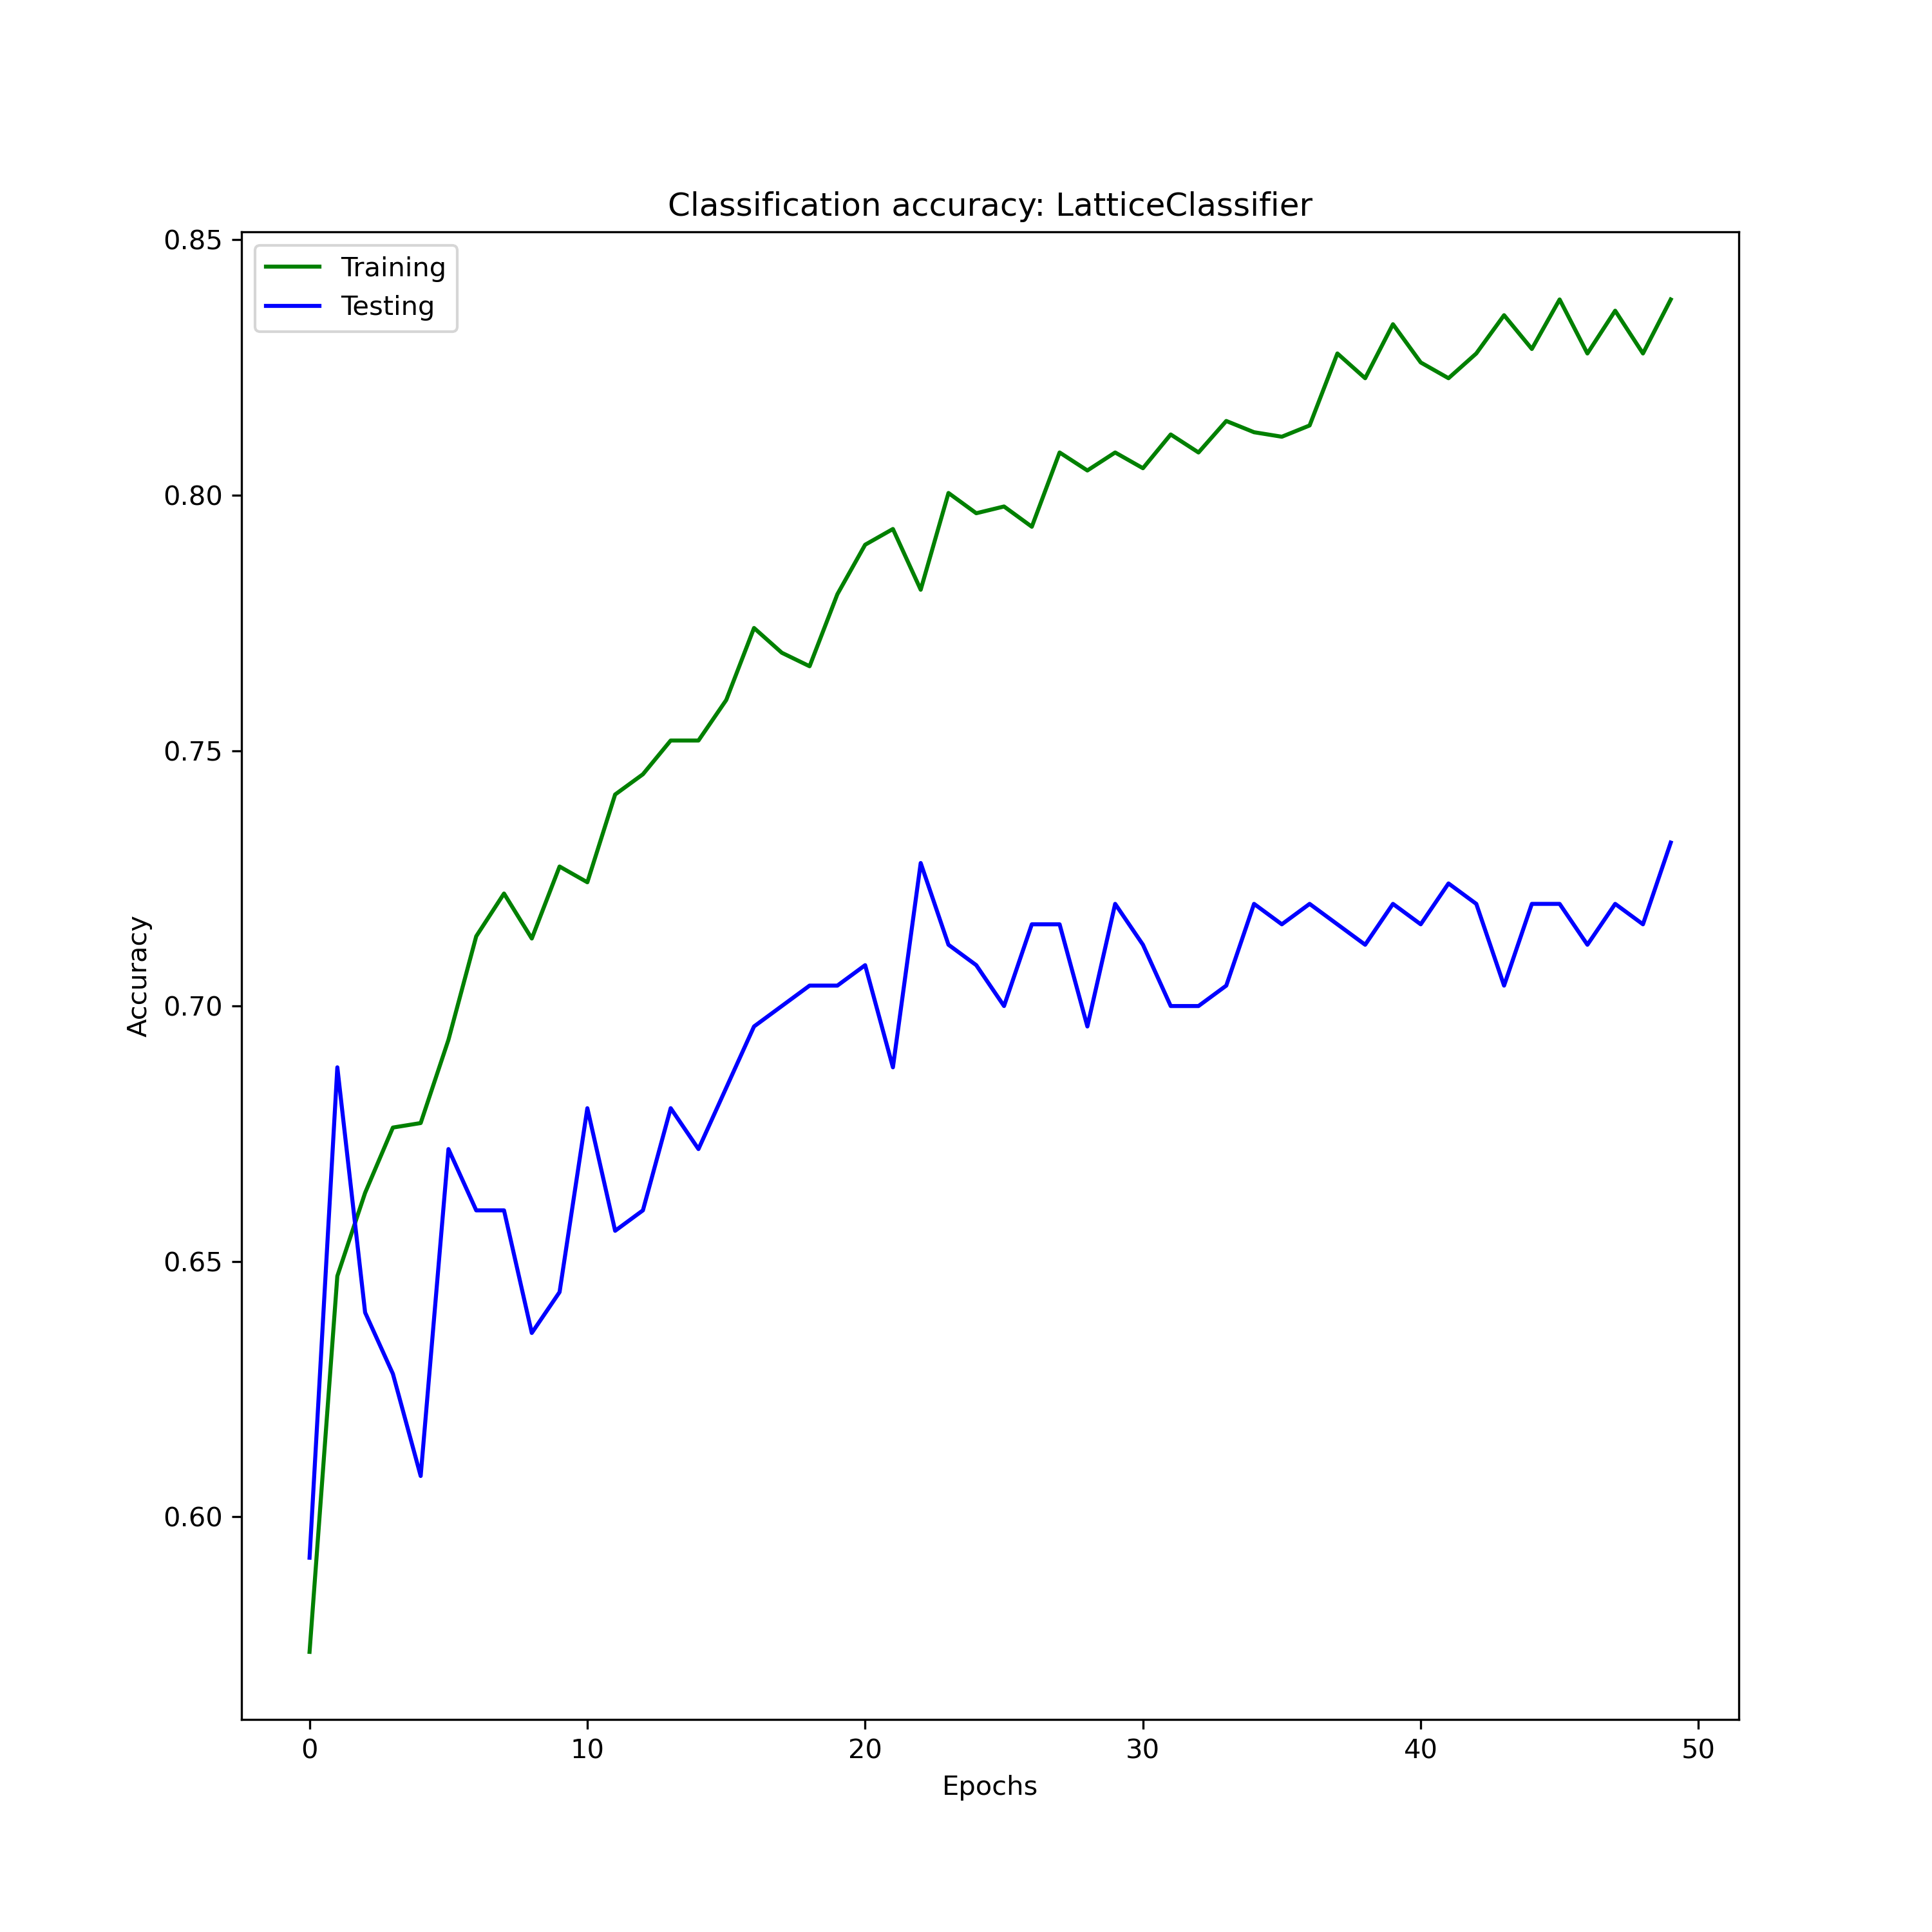
\includegraphics[width=0.49\textwidth]{lattice_accuracy.png}
    \vspace{0.2cm}
    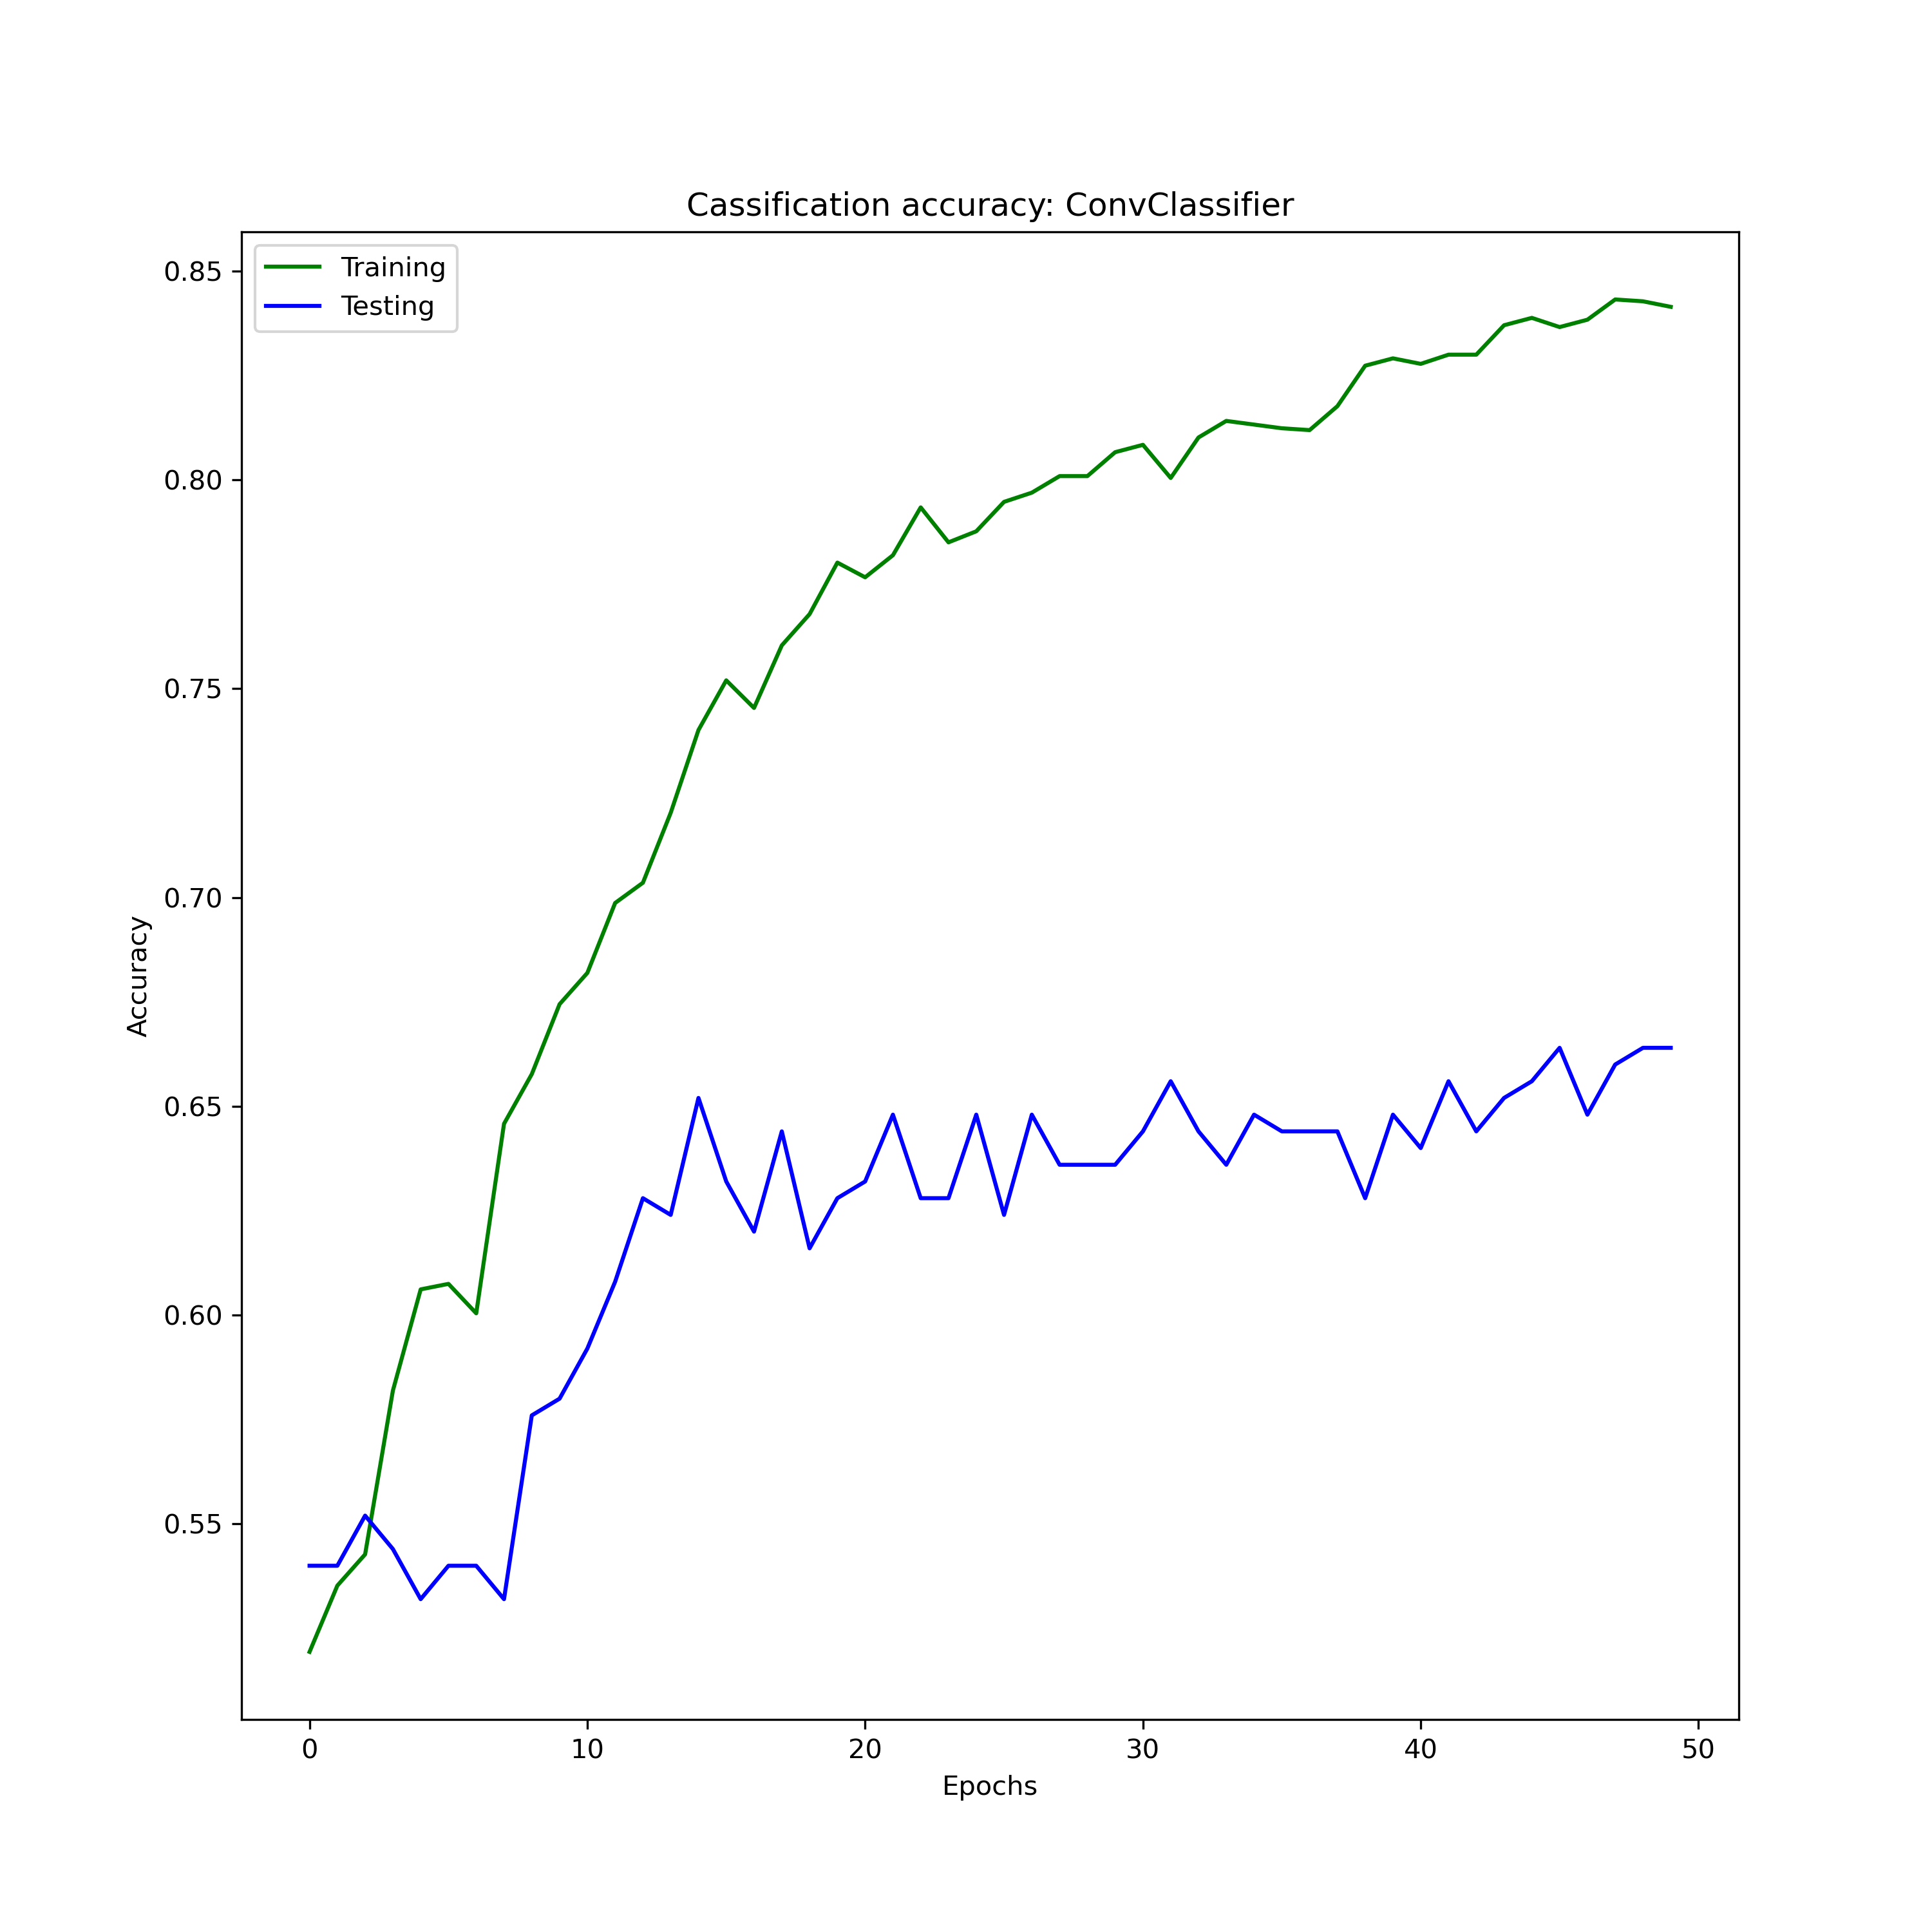
\includegraphics[width=0.49\textwidth]{conv_accuracy.png}
    \end{center}
    
\end{figure}

We use a small portion of the Princeton ModelNet
dataset~\cite{zhirong_wu_3d_2015} as a source of finite
metric spaces. This dataset consists of hundreds of 3-dimensional CAD models
representing objects from 10 classes. We select two of the classes and sample
points from the 3D models to produce finite metric spaces embedded in $\R^3$.
We then compute the corresponding multidimensional persistence modules, from
which we produce features used as an input to a convolutional neural net
classifier.

The pipline thus begins with a 3D polyhedral model, of which $3000$ vertices are sampled to produce a point
cloud in $\R^3$. This point cloud then produces a bifiltered simplicial complex,
whose persistent homology we calculate using
RIVET~\cite{lesnick_interactive_2015}, sampled at a discrete grid of $40 \times
40$ points, producing lattice-indexed signals given by the Hilbert function and
the multi-graded Betti numbers $\xi_0, \xi_1, \xi_2$--four features in total. These are then passed to the classifier, which
produces a class prediction, in this case either ``sofa'' or ``monitor.''

As the filter function on these data sets, we use the \introduce{codensity} function
\[\rho_{\text{codense}}(x;k) = \frac{1}{\frac{1}{k} \sum_{y \in N_k(x)}
    d(x,y)},\]
where $N_k(x)$ is the set of the $k$ nearest neighbors to $x$.

% This is the
% \introduce{codensity} filtration, so named because the points in the densest
% regions of $\mathcal M$ will appear first.

% A folk theorem is that the
% two-parameter persistent homology of a Rips/codensity bifiltration is stable
% under non-Hausdorff perturbations: \textit{the (Rips) persistent homology of a
%   point sample and another obtained by adding a small number of points at random
% are close with respect to the interleaving distance}.

We compare the performance of two convolutional networks on this classification
task. One uses the lattice-convolution based layers described in
Section~\ref{sec:latticeCNN}, and the other uses standard convolutional layers.
Each has three convolutional layers followed by three fully connected layers.
The lattice-based convolution layers are of the form $\text{MeetConv}(x) +
\text{JoinConv}(x)$. All convolution kernels have dimension $4 \times 4$, hidden
convolution layers have 16 features, and the final convolution has 8 features.
The fully connected layers have 32 features at each inner layer.
The networks are trained using the Adam gradient algorithm with learning rate
$0.001$ for 50 epochs. We reserve 10\% of the data for testing. Results are
shown in Figure~\ref{fig:comparison}.

The lattice-based convolution and classical convolution networks perform
similarly on the training set. However, the lattice convolution network's
predictions generalize more accurately to the testing set ($\approx 7\%$ improvement in testing accuracy).
This improvement is  at the expense of more variability in performance during
training. %noisy training as well as dramatically increased training time.  
%% more discussion of what the data actually looks like

\section{Discussion}
Our proposed featurization for persistence modules is rather naive, but well
adapted to the use of lattice convolutions as a data processing method. The
lattice convolutional neural network shows promise as a method for classifying
features arising from a multiparameter persistence module. The algebraic
perspective on partially ordered sets, exemplified by lattices, may also offer
approaches to featurizing more complex invariants of persistence modules. In
particular, the incidence algebra may offer a natural way to represent the rank
invariant~\cite{carlsson_theory_2009} in a way amenable to convolution-like
operations.
We hope with these brief experiments to inspire further work on featurizing
multidimensional persistence for use in machine learning algorithms.
% anything else?

\bibliographystyle{plain}
\bibliography{latticenn}

\end{document}
